% Options for packages loaded elsewhere
\PassOptionsToPackage{unicode}{hyperref}
\PassOptionsToPackage{hyphens}{url}
%
\documentclass[
  12pt,
]{article}
\usepackage{lmodern}
\usepackage{amsmath}
\usepackage{ifxetex,ifluatex}
\ifnum 0\ifxetex 1\fi\ifluatex 1\fi=0 % if pdftex
  \usepackage[T1]{fontenc}
  \usepackage[utf8]{inputenc}
  \usepackage{textcomp} % provide euro and other symbols
  \usepackage{amssymb}
\else % if luatex or xetex
  \usepackage{unicode-math}
  \defaultfontfeatures{Scale=MatchLowercase}
  \defaultfontfeatures[\rmfamily]{Ligatures=TeX,Scale=1}
  \setmainfont[]{Times New Roman}
\fi
% Use upquote if available, for straight quotes in verbatim environments
\IfFileExists{upquote.sty}{\usepackage{upquote}}{}
\IfFileExists{microtype.sty}{% use microtype if available
  \usepackage[]{microtype}
  \UseMicrotypeSet[protrusion]{basicmath} % disable protrusion for tt fonts
}{}
\makeatletter
\@ifundefined{KOMAClassName}{% if non-KOMA class
  \IfFileExists{parskip.sty}{%
    \usepackage{parskip}
  }{% else
    \setlength{\parindent}{0pt}
    \setlength{\parskip}{6pt plus 2pt minus 1pt}}
}{% if KOMA class
  \KOMAoptions{parskip=half}}
\makeatother
\usepackage{xcolor}
\IfFileExists{xurl.sty}{\usepackage{xurl}}{} % add URL line breaks if available
\IfFileExists{bookmark.sty}{\usepackage{bookmark}}{\usepackage{hyperref}}
\hypersetup{
  pdftitle={PFAS Levels in North Carolina},
  pdfauthor={Karly Nocera and Tay Holliday},
  hidelinks,
  pdfcreator={LaTeX via pandoc}}
\urlstyle{same} % disable monospaced font for URLs
\usepackage[margin=2.54cm]{geometry}
\usepackage{color}
\usepackage{fancyvrb}
\newcommand{\VerbBar}{|}
\newcommand{\VERB}{\Verb[commandchars=\\\{\}]}
\DefineVerbatimEnvironment{Highlighting}{Verbatim}{commandchars=\\\{\}}
% Add ',fontsize=\small' for more characters per line
\usepackage{framed}
\definecolor{shadecolor}{RGB}{248,248,248}
\newenvironment{Shaded}{\begin{snugshade}}{\end{snugshade}}
\newcommand{\AlertTok}[1]{\textcolor[rgb]{0.94,0.16,0.16}{#1}}
\newcommand{\AnnotationTok}[1]{\textcolor[rgb]{0.56,0.35,0.01}{\textbf{\textit{#1}}}}
\newcommand{\AttributeTok}[1]{\textcolor[rgb]{0.77,0.63,0.00}{#1}}
\newcommand{\BaseNTok}[1]{\textcolor[rgb]{0.00,0.00,0.81}{#1}}
\newcommand{\BuiltInTok}[1]{#1}
\newcommand{\CharTok}[1]{\textcolor[rgb]{0.31,0.60,0.02}{#1}}
\newcommand{\CommentTok}[1]{\textcolor[rgb]{0.56,0.35,0.01}{\textit{#1}}}
\newcommand{\CommentVarTok}[1]{\textcolor[rgb]{0.56,0.35,0.01}{\textbf{\textit{#1}}}}
\newcommand{\ConstantTok}[1]{\textcolor[rgb]{0.00,0.00,0.00}{#1}}
\newcommand{\ControlFlowTok}[1]{\textcolor[rgb]{0.13,0.29,0.53}{\textbf{#1}}}
\newcommand{\DataTypeTok}[1]{\textcolor[rgb]{0.13,0.29,0.53}{#1}}
\newcommand{\DecValTok}[1]{\textcolor[rgb]{0.00,0.00,0.81}{#1}}
\newcommand{\DocumentationTok}[1]{\textcolor[rgb]{0.56,0.35,0.01}{\textbf{\textit{#1}}}}
\newcommand{\ErrorTok}[1]{\textcolor[rgb]{0.64,0.00,0.00}{\textbf{#1}}}
\newcommand{\ExtensionTok}[1]{#1}
\newcommand{\FloatTok}[1]{\textcolor[rgb]{0.00,0.00,0.81}{#1}}
\newcommand{\FunctionTok}[1]{\textcolor[rgb]{0.00,0.00,0.00}{#1}}
\newcommand{\ImportTok}[1]{#1}
\newcommand{\InformationTok}[1]{\textcolor[rgb]{0.56,0.35,0.01}{\textbf{\textit{#1}}}}
\newcommand{\KeywordTok}[1]{\textcolor[rgb]{0.13,0.29,0.53}{\textbf{#1}}}
\newcommand{\NormalTok}[1]{#1}
\newcommand{\OperatorTok}[1]{\textcolor[rgb]{0.81,0.36,0.00}{\textbf{#1}}}
\newcommand{\OtherTok}[1]{\textcolor[rgb]{0.56,0.35,0.01}{#1}}
\newcommand{\PreprocessorTok}[1]{\textcolor[rgb]{0.56,0.35,0.01}{\textit{#1}}}
\newcommand{\RegionMarkerTok}[1]{#1}
\newcommand{\SpecialCharTok}[1]{\textcolor[rgb]{0.00,0.00,0.00}{#1}}
\newcommand{\SpecialStringTok}[1]{\textcolor[rgb]{0.31,0.60,0.02}{#1}}
\newcommand{\StringTok}[1]{\textcolor[rgb]{0.31,0.60,0.02}{#1}}
\newcommand{\VariableTok}[1]{\textcolor[rgb]{0.00,0.00,0.00}{#1}}
\newcommand{\VerbatimStringTok}[1]{\textcolor[rgb]{0.31,0.60,0.02}{#1}}
\newcommand{\WarningTok}[1]{\textcolor[rgb]{0.56,0.35,0.01}{\textbf{\textit{#1}}}}
\usepackage{longtable,booktabs}
\usepackage{calc} % for calculating minipage widths
% Correct order of tables after \paragraph or \subparagraph
\usepackage{etoolbox}
\makeatletter
\patchcmd\longtable{\par}{\if@noskipsec\mbox{}\fi\par}{}{}
\makeatother
% Allow footnotes in longtable head/foot
\IfFileExists{footnotehyper.sty}{\usepackage{footnotehyper}}{\usepackage{footnote}}
\makesavenoteenv{longtable}
\usepackage{graphicx}
\makeatletter
\def\maxwidth{\ifdim\Gin@nat@width>\linewidth\linewidth\else\Gin@nat@width\fi}
\def\maxheight{\ifdim\Gin@nat@height>\textheight\textheight\else\Gin@nat@height\fi}
\makeatother
% Scale images if necessary, so that they will not overflow the page
% margins by default, and it is still possible to overwrite the defaults
% using explicit options in \includegraphics[width, height, ...]{}
\setkeys{Gin}{width=\maxwidth,height=\maxheight,keepaspectratio}
% Set default figure placement to htbp
\makeatletter
\def\fps@figure{htbp}
\makeatother
\setlength{\emergencystretch}{3em} % prevent overfull lines
\providecommand{\tightlist}{%
  \setlength{\itemsep}{0pt}\setlength{\parskip}{0pt}}
\setcounter{secnumdepth}{5}
\ifluatex
  \usepackage{selnolig}  % disable illegal ligatures
\fi

\title{PFAS Levels in North Carolina}
\usepackage{etoolbox}
\makeatletter
\providecommand{\subtitle}[1]{% add subtitle to \maketitle
  \apptocmd{\@title}{\par {\large #1 \par}}{}{}
}
\makeatother
\subtitle{\url{https://github.com/kn134/EDAFinal_PFAS.git}}
\author{Karly Nocera and Tay Holliday}
\date{4/26/2021}

\begin{document}
\maketitle

\newpage
\tableofcontents 
\newpage
\listoftables 
\newpage
\listoffigures 
\newpage

\begin{Shaded}
\begin{Highlighting}[]
\CommentTok{\#sets the default values of chunk options}
\NormalTok{knitr}\SpecialCharTok{::}\NormalTok{opts\_chunk}\SpecialCharTok{$}\FunctionTok{set}\NormalTok{(}\AttributeTok{echo =} \ConstantTok{FALSE}\NormalTok{, }\AttributeTok{fig.width =} \DecValTok{10}\NormalTok{, }\AttributeTok{fig.height =} \DecValTok{10}\NormalTok{)}
\end{Highlighting}
\end{Shaded}

\begin{itemize}
\tightlist
\item
  Knitting commands in code chunks:
\item
  \texttt{include\ =\ FALSE} - code is run, but neither code nor results
  appear in knitted file
\item
  \texttt{echo\ =\ FALSE} - code not included in knitted file, but
  results are
\item
  \texttt{eval\ =\ FALSE} - code is not run in the knitted file
\item
  \texttt{message\ =\ FALSE} - messages do not appear in knitted file
\item
  \texttt{warning\ =\ FALSE} - warnings do not appear\ldots{}
\item
  \texttt{fig.cap\ =\ "..."} - adds a caption to graphical results
\end{itemize}

\hypertarget{rationale-and-research-questions}{%
\section{Rationale and Research
Questions}\label{rationale-and-research-questions}}

The purpose of this study was to synthesize and analyze the findings of
local water quality samples measuring a group of emerging contaminants,
PFAS (per- and polyfluoroalkyl substances). The two datasets from DEQ
(2018 Emerging Compounds Monitoring Reports of various watersheds and
public water supply (PWS) reservoirs and the 2019 wastewater treatment
plant (WWTP) samples) were chosen as the only publicly-available
datasets on local PFAS levels. The sample locations and variables were
pre-determined by the study, but these datasets reflect locations and
variables pertaining to the levels of various PFAS analytes in the
drinking water and water bodies associated with 2.7 million North
Carolina residents.

Our study aims to explore and analyze this data in order to begin
building the larger story of local contamination and identify areas of
concern that need further investigation. To do so, we answered the
following questions:

\begin{enumerate}
\def\labelenumi{\arabic{enumi}.}
\tightlist
\item
  Occurence
\end{enumerate}

\begin{itemize}
\tightlist
\item
  What are the most abundant analytes present?
\item
  Which sites have analytes exceeding health advisory levels?
\item
  What chain lengths are most abundant and present?
\item
  What portion of total PFAS are PFOA and PFOS?
\end{itemize}

\begin{enumerate}
\def\labelenumi{\arabic{enumi}.}
\setcounter{enumi}{1}
\tightlist
\item
  Distribution
\end{enumerate}

\begin{itemize}
\tightlist
\item
  Are there bodies of water with concerningly high levels of PFAS that
  aren't commonly discussed?
\item
  How does total PFAS change over time?
\end{itemize}

\begin{enumerate}
\def\labelenumi{\arabic{enumi}.}
\setcounter{enumi}{2}
\tightlist
\item
  Unreported / Further Investigation
\end{enumerate}

\begin{itemize}
\tightlist
\item
  What is the highest reporting limit for each analyte?
\item
  How many samples had reporting limits above health advisory levels?
\item
  What percentage of total unreported results were below health advisory
  limits?
\end{itemize}

\newpage

\hypertarget{dataset-information}{%
\section{Dataset Information}\label{dataset-information}}

The two datasets were downloaded from North Carolina DEQ:
\href{https://deq.nc.gov/about/divisions/water-resources/water-resources-science-and-data/water-sciences-home-page/emerging}{2018
Analytical Results for PFAS Screening of Select Public Water Supply
(PWS) Reservoirs} and
\href{https://files.nc.gov/ncdeq/Water\%20Resources/GIS/Data/Emerging_Compounds_Mastersheet_12202019.pdf}{2019
publicaly owned utilities with pretreatment programs (POTWs) and
industrial dischargers with state permits}. Respective to their type of
site, both datasets contained site location, sample date, PFAS analyte
levels (nanograms per liter (ng/L) or equivalent parts per trillion
(ppt)), and lab qualifiers/reporting limits. To substantiate this
analysis, we incorporated a manually created csv file identifying the
latitude and longitude of sample sites, and researched analytes' chain
length (short or long).

Due to the nature of their original format, both datasets needed
extensive cleaning prior to importing to R and further exploration and
analysis. The POTW data was originally in a PDF and first needed to be
converted (using SmallPDF tool) to an excel spreadsheet. These values
were then manually moved intoa dataset layout (column headings, rows for
each analyte sampled). The PWS dataset was already a csv dataset. For
both, analytes with dashes (-) needed to be replaced with a different
character (.) in order to read into R and column names were changed to
be consistent with other. The lab qualifiers were split so that there
was a unique column of numeric reporting limits and in PWS the
``results'' value was deleted because it was actually the reporting
limit and not a result, despite being originally in that column
(indicated with corresponding lab qualifier characters).

Once these three datasets were imported into R Studio, both POTW and PWS
needed the ``sample date'' column formatted as a date class and
unnecessary columns were removed. To pivot each wider for future use,
their reporting limit column was removed and then each pivoted wider so
that each analyte became a column with its corresponding parts per
trillion measurement. We then mutated both datasets to create columns
for Total PFAS, the sum of PFOA and PFOS (due to health advisory
regulation), the sum of all short-chained PFAS, and the sum of all
long-chained PFAS.

To create a column for chain length in the original long datasets, we
used a function to determine if each analyte was short or long, adding
the result in the column. Then, both were joined to the imported
location dataset so each site had a longitude and latitude. These
cleaned files were then saved in the
Data\textgreater\textgreater Processed folder as csv.

\begin{longtable}[]{@{}ll@{}}
\toprule
\begin{minipage}[b]{(\columnwidth - 1\tabcolsep) * \real{0.52}}\raggedright
Data Structure\strut
\end{minipage} &
\begin{minipage}[b]{(\columnwidth - 1\tabcolsep) * \real{0.48}}\raggedright
Value\strut
\end{minipage}\tabularnewline
\midrule
\endhead
\begin{minipage}[t]{(\columnwidth - 1\tabcolsep) * \real{0.52}}\raggedright
Variables\strut
\end{minipage} &
\begin{minipage}[t]{(\columnwidth - 1\tabcolsep) * \real{0.48}}\raggedright
Site, Analyte, ppt, Total PFAS, Sum PFOA PFOS, short-chain, long-chain,
latitude, longitude\strut
\end{minipage}\tabularnewline
\begin{minipage}[t]{(\columnwidth - 1\tabcolsep) * \real{0.52}}\raggedright
Units\strut
\end{minipage} &
\begin{minipage}[t]{(\columnwidth - 1\tabcolsep) * \real{0.48}}\raggedright
parts per trillion (ppt) or equivalent nanograms per liter (ng/L)\strut
\end{minipage}\tabularnewline
\begin{minipage}[t]{(\columnwidth - 1\tabcolsep) * \real{0.52}}\raggedright
Range\strut
\end{minipage} &
\begin{minipage}[t]{(\columnwidth - 1\tabcolsep) * \real{0.48}}\raggedright
2650 (POTW) and 552 (PWS)\strut
\end{minipage}\tabularnewline
\begin{minipage}[t]{(\columnwidth - 1\tabcolsep) * \real{0.52}}\raggedright
Skew\strut
\end{minipage} &
\begin{minipage}[t]{(\columnwidth - 1\tabcolsep) * \real{0.48}}\raggedright
14.28 (POTW) and 3.56 (PWS)\strut
\end{minipage}\tabularnewline
\begin{minipage}[t]{(\columnwidth - 1\tabcolsep) * \real{0.52}}\raggedright
Kertosis\strut
\end{minipage} &
\begin{minipage}[t]{(\columnwidth - 1\tabcolsep) * \real{0.48}}\raggedright
254.5 (POTW) and 15.2 (PWS)\strut
\end{minipage}\tabularnewline
\begin{minipage}[t]{(\columnwidth - 1\tabcolsep) * \real{0.52}}\raggedright
Links to Data Sources\strut
\end{minipage} &
\begin{minipage}[t]{(\columnwidth - 1\tabcolsep) * \real{0.48}}\raggedright
\href{https://deq.nc.gov/about/divisions/water-resources/water-resources-science-and-data/water-sciences-home-page/emerging}{2018
PWS} and
\href{https://files.nc.gov/ncdeq/Water\%20Resources/GIS/Data/Emerging_Compounds_Mastersheet_12202019.pdf}{2019
POTWs}\strut
\end{minipage}\tabularnewline
\bottomrule
\end{longtable}

\newpage

\hypertarget{exploratory-analysis}{%
\section{Exploratory Analysis}\label{exploratory-analysis}}

\hypertarget{unique-analytes}{%
\subsection{Unique analytes}\label{unique-analytes}}

45 unique analytes were found in POTW samples and 23 in PWS. The
following two tables display the most abundant analytes found in each
set of site samples.

\begin{longtable}[]{@{}lr@{}}
\caption{Top 10 Abundant Analytes in POTW}\tabularnewline
\toprule
Analyte & Count\tabularnewline
\midrule
\endfirsthead
\toprule
Analyte & Count\tabularnewline
\midrule
\endhead
PFOA & 74\tabularnewline
PFHxA & 73\tabularnewline
PFOS & 73\tabularnewline
PFHpA & 68\tabularnewline
PFPeA & 54\tabularnewline
PFNA & 45\tabularnewline
PFDA & 42\tabularnewline
PFHxS & 33\tabularnewline
PFBS & 26\tabularnewline
PFBA & 25\tabularnewline
\bottomrule
\end{longtable}

\begin{longtable}[]{@{}lr@{}}
\caption{Top 10 Abundant Analytes in PWS}\tabularnewline
\toprule
Analyte & Count\tabularnewline
\midrule
\endfirsthead
\toprule
Analyte & Count\tabularnewline
\midrule
\endhead
PFPeA & 17\tabularnewline
PFHxA & 15\tabularnewline
PFHpA & 14\tabularnewline
PFBA & 10\tabularnewline
PFOS & 8\tabularnewline
PFOA & 4\tabularnewline
PFHxS & 2\tabularnewline
4.2 & 0\tabularnewline
6.2 & 0\tabularnewline
8.2 & 0\tabularnewline
\bottomrule
\end{longtable}

\hypertarget{number-of-samples-with-each-analyte}{%
\subsection{Number of samples with each
analyte}\label{number-of-samples-with-each-analyte}}

The following histograms visualize the number of samples of each
analyte. Same as above, the abundnace indicates which PFAS are most
commonly present. This is relevant for regulation and possibly tracking
contaminant sources.

\begin{figure}

\includegraphics{PFAS_FinalProject_files/figure-latex/plotN-1} \hfill{}

\caption{Number of Samples in POTW}\label{fig:plotN}
\end{figure}
\begin{figure}

\includegraphics{PFAS_FinalProject_files/figure-latex/plotW-1} \hfill{}

\caption{Number of Samples in PWS}\label{fig:plotW}
\end{figure}

\hypertarget{number-of-select-analytes-by-level}{%
\subsection{Number of Select Analytes by
Level}\label{number-of-select-analytes-by-level}}

The following histograms visualize the number of samples of PFAS levels.
The abundnace indicates which PFAS are most commonly present and which
analytes have a high count at higher levels (ppt). This is relevant for
regulation and possibly tracking contaminant sources.

\begin{verbatim}
## Warning: Removed 237 rows containing non-finite values (stat_bin).
\end{verbatim}

\begin{verbatim}
## Warning: Removed 18 row(s) containing missing values (geom_path).
\end{verbatim}

\begin{figure}

\includegraphics{PFAS_FinalProject_files/figure-latex/unnamed-chunk-4-1} \hfill{}

\caption{Number of Samples by Level in POTW}\label{fig:unnamed-chunk-4}
\end{figure}

\begin{verbatim}
## Warning: Removed 1209 rows containing non-finite values (stat_bin).
\end{verbatim}

\begin{verbatim}
## Warning: Removed 12 row(s) containing missing values (geom_path).
\end{verbatim}

\begin{figure}

\includegraphics{PFAS_FinalProject_files/figure-latex/unnamed-chunk-5-1} \hfill{}

\caption{Number of Samples by Level in PWS}\label{fig:unnamed-chunk-5}
\end{figure}

\hypertarget{density-ridge-lines-of-select-analytes}{%
\subsection{Density ridge lines of select
analytes}\label{density-ridge-lines-of-select-analytes}}

A closer look the count of analyte samples by value (ppt) indicates
which analytes have frequently high values. This is valuable knowledge
to begin analyzing whether high levels are an isolated event or
consistently high.

\begin{verbatim}
## Picking joint bandwidth of 9.19
\end{verbatim}

\begin{verbatim}
## Warning: Removed 226 rows containing non-finite values (stat_density_ridges).
\end{verbatim}

\begin{figure}

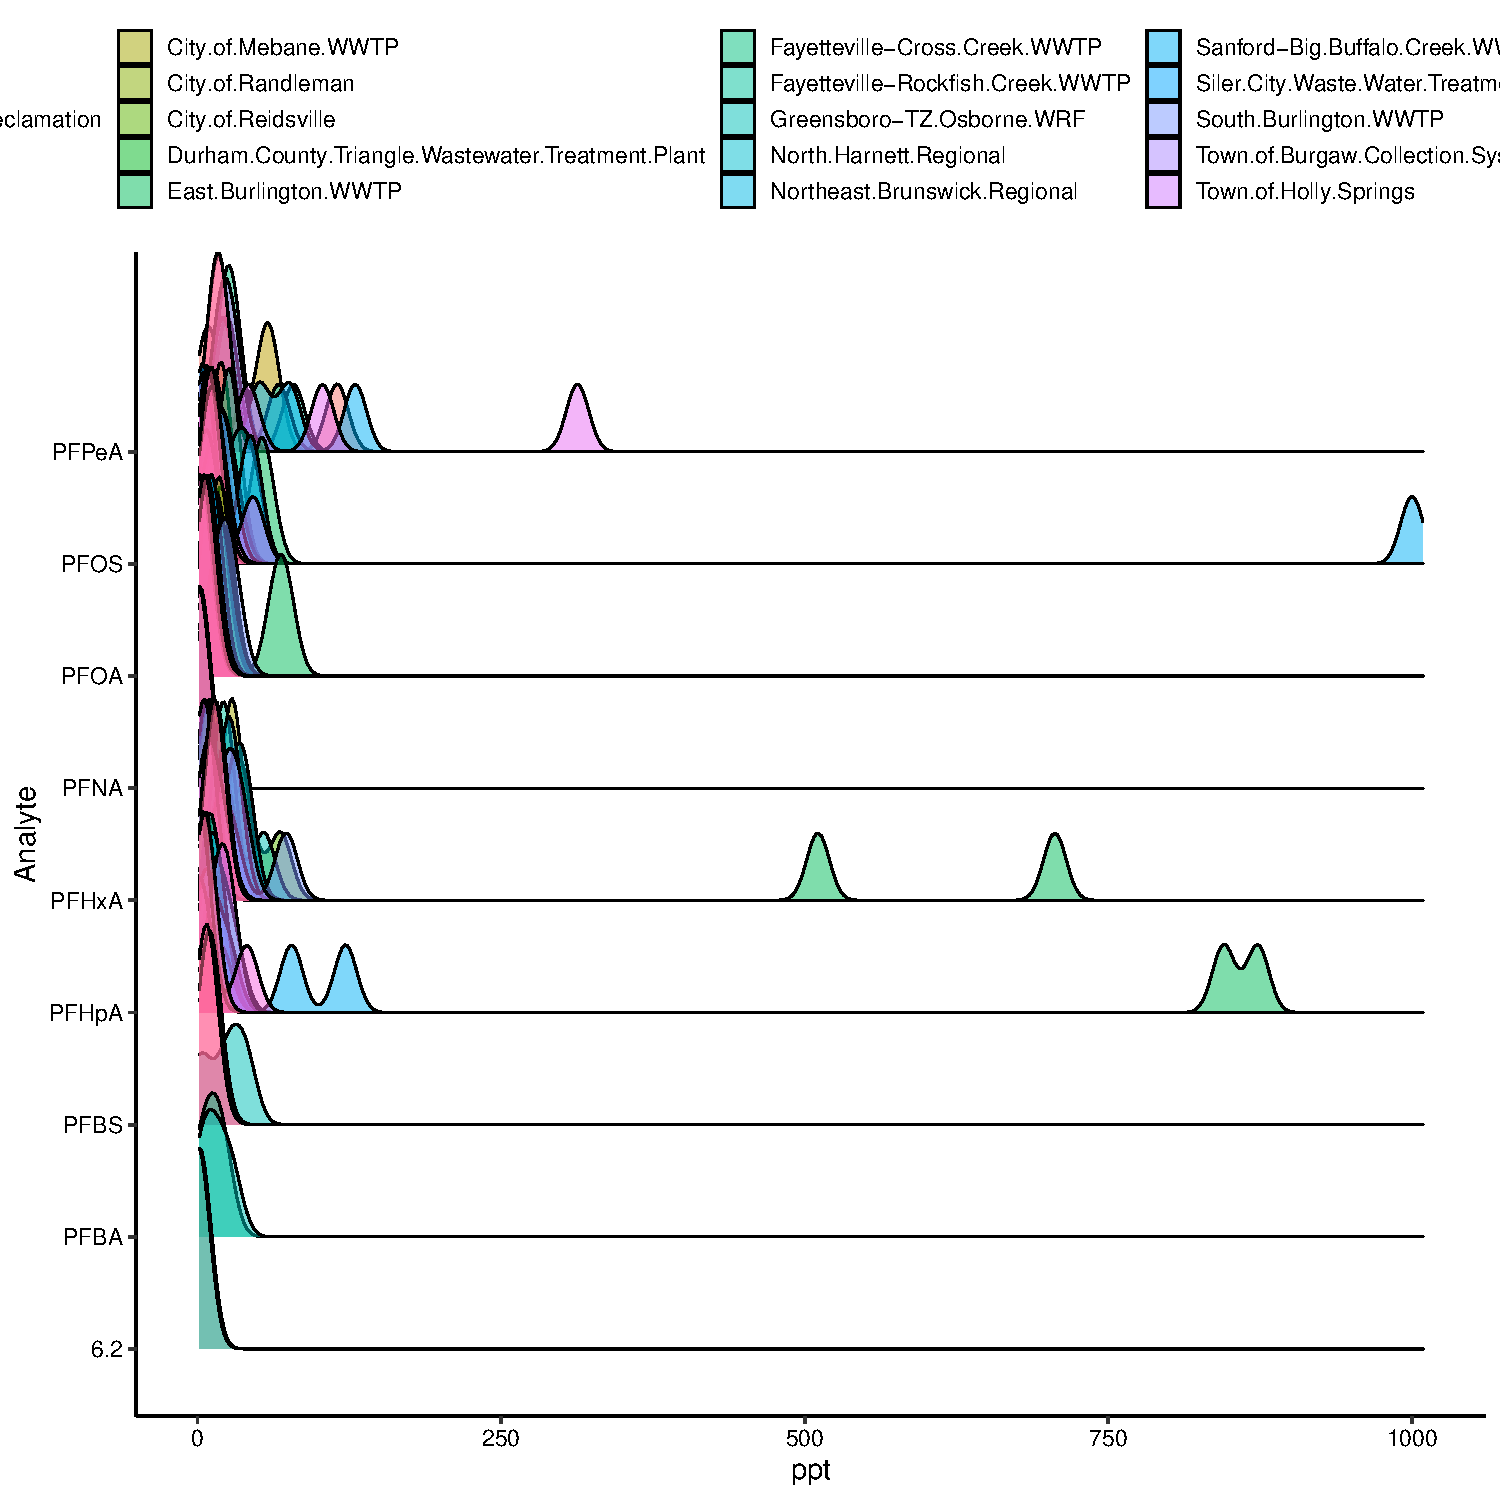
\includegraphics{PFAS_FinalProject_files/figure-latex/unnamed-chunk-6-1} \hfill{}

\caption{Density Ridges of Select Analytes by Level in POTW}\label{fig:unnamed-chunk-6}
\end{figure}

\begin{verbatim}
## Picking joint bandwidth of 17.5
\end{verbatim}

\begin{verbatim}
## Warning: Removed 1209 rows containing non-finite values (stat_density_ridges).
\end{verbatim}

\begin{figure}

\includegraphics{PFAS_FinalProject_files/figure-latex/unnamed-chunk-7-1} \hfill{}

\caption{Density Ridges of Select Analytes by Level in PWS}\label{fig:unnamed-chunk-7}
\end{figure}

\hypertarget{distribution-of-pfoa-and-pfos-samples}{%
\subsection{Distribution of PFOA and PFOS
samples}\label{distribution-of-pfoa-and-pfos-samples}}

Violin plots illustrating the distribution of PFOA and PFOS in both
sample site types indicate the quartiles of both analytes. This is
important for understanding the PFAS levels where the bulk of samples
occured.

\begin{verbatim}
## Warning: Removed 17 rows containing non-finite values (stat_ydensity).
\end{verbatim}

\begin{verbatim}
## Warning in regularize.values(x, y, ties, missing(ties), na.rm = na.rm):
## collapsing to unique 'x' values
\end{verbatim}

\begin{figure}

\includegraphics{PFAS_FinalProject_files/figure-latex/unnamed-chunk-8-1} \hfill{}

\caption{Violin Plots of PFOA and PFOS in POTW}\label{fig:unnamed-chunk-8}
\end{figure}

\begin{verbatim}
## Warning: Removed 268 rows containing non-finite values (stat_ydensity).
\end{verbatim}

\begin{verbatim}
## Warning in regularize.values(x, y, ties, missing(ties), na.rm = na.rm):
## collapsing to unique 'x' values
\end{verbatim}

\begin{figure}

\includegraphics{PFAS_FinalProject_files/figure-latex/unnamed-chunk-9-1} \hfill{}

\caption{Violin Plots of PFOA and PFOS in PWS}\label{fig:unnamed-chunk-9}
\end{figure}

\hypertarget{pfoapfos-exceeding-health-advisory-in-potw}{%
\subsection{PFOA/PFOS exceeding health advisory in
POTW}\label{pfoapfos-exceeding-health-advisory-in-potw}}

These tables shows the three sites that had the sum of PFOA and PFOS
over 70ppt (EPA's health advisory level) during the three-month testing
samples.

\begin{longtable}[]{@{}lrrrl@{}}
\caption{Sites Exceeding EPA Health Advisory Limit}\tabularnewline
\toprule
Site & PFOA & PFOS & Sum & Sample.Date\tabularnewline
\midrule
\endfirsthead
\toprule
Site & PFOA & PFOS & Sum & Sample.Date\tabularnewline
\midrule
\endhead
City.of.Raeford & NA & 124.0 & 124.0 & 2019-09-16\tabularnewline
City.of.Raeford & NA & 73.6 & 73.6 & 2019-08-05\tabularnewline
City.of.Raeford & NA & NA & 0.0 & 2019-07-15\tabularnewline
East.Burlington.WWTP & 10.8 & 12.5 & 23.3 & 2019-09-17\tabularnewline
East.Burlington.WWTP & 64.6 & 56.4 & 121.0 & 2019-08-06\tabularnewline
East.Burlington.WWTP & 73.0 & 49.8 & 122.8 & 2019-07-16\tabularnewline
Sanford-Big.Buffalo.Creek.WWTP & 11.0 & 1000.0 & 1011.0 &
2019-09-04\tabularnewline
Sanford-Big.Buffalo.Creek.WWTP & 11.5 & 40.8 & 52.3 &
2019-08-06\tabularnewline
Sanford-Big.Buffalo.Creek.WWTP & 11.6 & 46.3 & 57.9 &
2019-07-08\tabularnewline
\bottomrule
\end{longtable}

\hypertarget{maximum-reporting-limits-per-analyte}{%
\subsection{Maximum reporting limits per
analyte}\label{maximum-reporting-limits-per-analyte}}

If an analyte was measured below a reporting limit (ppt), it was not
reported. Particularly high reporting limits are concerning because it
indicates that there are sites that may have high levels of PFAS that
are overlooked. While there is no specific value that is ``too'' high,
long-chain PFAS are a known health risk at lower levels (e.g., 8ppt).
These tables indicate the maximum reporting limits that occured for each
analyte sampled.

\begin{longtable}[]{@{}lr@{}}
\caption{Max. Reporting Limits of Each Analyte in POTW}\tabularnewline
\toprule
Analyte & Max. Reporting Limit\tabularnewline
\midrule
\endfirsthead
\toprule
Analyte & Max. Reporting Limit\tabularnewline
\midrule
\endhead
N.EtFOSAA & 1900.00\tabularnewline
N.MeFOSAA & 1900.00\tabularnewline
PFDoA & 420.00\tabularnewline
PFBA & 380.00\tabularnewline
PFDA & 380.00\tabularnewline
PFTeA & 380.00\tabularnewline
PFTriA & 380.00\tabularnewline
PFUnA & 380.00\tabularnewline
HFPO.DA & 354.62\tabularnewline
4.2 & 333.00\tabularnewline
PFHxDA & 210.00\tabularnewline
PFNA & 210.00\tabularnewline
PFODA & 210.00\tabularnewline
PFDS & 200.00\tabularnewline
PFHpS & 170.00\tabularnewline
PFNS & 170.00\tabularnewline
PFOA & 170.00\tabularnewline
PFOSA & 170.00\tabularnewline
PFBS & 120.00\tabularnewline
PFHpA & 120.00\tabularnewline
PFHxA & 120.00\tabularnewline
PFHxS & 120.00\tabularnewline
PFOS & 120.00\tabularnewline
PFPeA & 120.00\tabularnewline
PFPeS & 120.00\tabularnewline
6.2 & 89.60\tabularnewline
8.2 & 85.00\tabularnewline
PFPrOPrA & 21.00\tabularnewline
N.MeFOSA & 18.90\tabularnewline
N.EtFOSA & 18.70\tabularnewline
N.EtFOSE & 9.43\tabularnewline
N.MeFOSE & 9.43\tabularnewline
Nafion.Byproduct.1 & 3.77\tabularnewline
PFECA.G & 3.77\tabularnewline
PFMOPrA & 3.77\tabularnewline
10.2 & 3.62\tabularnewline
Nafion.Byproduct.2 & 3.57\tabularnewline
PFMOBA & 3.57\tabularnewline
PF3OUdS & 3.55\tabularnewline
PFMOAA & 3.40\tabularnewline
PFO2HxA & 3.40\tabularnewline
PFO3OA & 3.40\tabularnewline
PFO4DA & 3.40\tabularnewline
ADONA & 1.89\tabularnewline
PF3ONS & 1.76\tabularnewline
\bottomrule
\end{longtable}

\begin{longtable}[]{@{}lr@{}}
\caption{Max. Reporting Limits of Each Analyte in PWS}\tabularnewline
\toprule
Analyte & Max. Reporting Limit\tabularnewline
\midrule
\endfirsthead
\toprule
Analyte & Max. Reporting Limit\tabularnewline
\midrule
\endhead
6.2 & 310\tabularnewline
PFUnA & 310\tabularnewline
NMeFOSAA & 160\tabularnewline
PFBA & 160\tabularnewline
PFDA & 160\tabularnewline
PFDoA & 160\tabularnewline
PFDS & 160\tabularnewline
PFNA & 160\tabularnewline
PFNS & 160\tabularnewline
PFTriA & 160\tabularnewline
8.2 & 83\tabularnewline
4.2 & 82\tabularnewline
PFHxA & 82\tabularnewline
PFOS & 80\tabularnewline
PFPeA & 80\tabularnewline
FOSA & 42\tabularnewline
HFPO.DA & 42\tabularnewline
PFBS & 42\tabularnewline
PFHpA & 42\tabularnewline
PFHpS & 42\tabularnewline
PFHxS & 42\tabularnewline
PFOA & 42\tabularnewline
PFPeS & 42\tabularnewline
\bottomrule
\end{longtable}

\newpage

\hypertarget{analysis}{%
\section{Analysis}\label{analysis}}

Each paragraph, accompanied by one or more visualizations, should
describe the major findings and how they relate to the question and
hypotheses.

\hypertarget{question-1-occurence}{%
\subsection{Question 1: Occurence}\label{question-1-occurence}}

\hypertarget{what-are-the-most-abundant-analytes-present}{%
\subsubsection{What are the most abundant analytes
present?}\label{what-are-the-most-abundant-analytes-present}}

FILL IN

\begin{verbatim}
## Warning: Removed 1303 rows containing missing values (position_stack).
\end{verbatim}

\begin{figure}

\includegraphics{PFAS_FinalProject_files/figure-latex/unnamed-chunk-13-1} \hfill{}

\caption{Analytes Present in POTW Sites}\label{fig:unnamed-chunk-13}
\end{figure}

\begin{verbatim}
## Warning: Removed 3166 rows containing missing values (position_stack).
\end{verbatim}

\begin{figure}

\includegraphics{PFAS_FinalProject_files/figure-latex/unnamed-chunk-14-1} \hfill{}

\caption{Analytes Present in PWS Sites}\label{fig:unnamed-chunk-14}
\end{figure}

\hypertarget{which-sites-have-analytes-exceeding-health-advisory-levels}{%
\subsubsection{Which sites have analytes exceeding health advisory
levels?}\label{which-sites-have-analytes-exceeding-health-advisory-levels}}

FILL IN

\begin{verbatim}
##  [1] City.of.Randleman                                
##  [2] Wallace.Regional.WWTP                            
##  [3] South.Burlington.WWTP                            
##  [4] Fayetteville-Cross.Creek.WWTP                    
##  [5] Greensboro-TZ.Osborne.WRF                        
##  [6] City.of.Raeford                                  
##  [7] City.of.High.Point.Eastside.WWTP                 
##  [8] Town.of.Holly.Springs                            
##  [9] City.of.Reidsville                               
## [10] City.of.Mebane.WWTP                              
## [11] Durham.County.Triangle.Wastewater.Treatment.Plant
## [12] Wilmington-James.A.Loughlin(Northside.WWTP       
## [13] Wilmington-M'Kean.Maffitt(Southside.WWTP         
## [14] Cit.of.Clinton-Norman.H.Larkins.WWTP             
## [15] City.of.Durham-South.Durham.Water.Reclamation    
## [16] Sanford-Big.Buffalo.Creek.WWTP                   
## [17] North.Harnett.Regional                           
## [18] Town.of.Ramseur.WWTP                             
## [19] Fayetteville-Rockfish.Creek.WWTP                 
## [20] Town.of.Rose.Hill.WWTP                           
## [21] East.Burlington.WWTP                             
## [22] City.of.Graham                                   
## [23] Northeast.Brunswick.Regional                     
## 27 Levels: Cary.Western.Wake.Regional.Water.Reclamation.Facility ...
\end{verbatim}

\begin{verbatim}
##  [1] City.of.Randleman                            
##  [2] Wallace.Regional.WWTP                        
##  [3] South.Burlington.WWTP                        
##  [4] City.of.Raeford                              
##  [5] City.of.Mebane.WWTP                          
##  [6] Cit.of.Clinton-Norman.H.Larkins.WWTP         
##  [7] City.of.Durham-South.Durham.Water.Reclamation
##  [8] Sanford-Big.Buffalo.Creek.WWTP               
##  [9] North.Harnett.Regional                       
## [10] Town.of.Ramseur.WWTP                         
## [11] Fayetteville-Rockfish.Creek.WWTP             
## [12] East.Burlington.WWTP                         
## [13] Northeast.Brunswick.Regional                 
## 27 Levels: Cary.Western.Wake.Regional.Water.Reclamation.Facility ...
\end{verbatim}

\begin{verbatim}
##  [1] HAWRIVATSR1713NRBYNUM                     
##  [2] NEWHOPECRKATSR1107NRBLANDS                
##  [3] NORTHEASTCRKATSR1100NRNELSON              
##  [4] NORTHEASTCRKATSR1731OKELLYCHURCHRDNRDURHAM
##  [5] HAWRIVBELOWJORDANDAMNRMONCURE             
##  [6] LakeBrandtatDamnearHillsdale              
##  [7] JORDANLAKEABOVESTINKINGCREEKNRPITTSBORONC 
##  [8] JORDANLAKEATMOUTHOFWHITEOAKCREEKNRSEAFORTH
##  [9] JORDANLAKEATNARROWSNEARBONSAL             
## [10] CaneCreekReservoiratDamnrOaks,NC          
## [11] KnapofReedsCreek                          
## 44 Levels: BlowingRockTownPond BooneASULake ... UniversityLakeatDamnrChapelHill,NC
\end{verbatim}

\begin{verbatim}
## [1] HAWRIVATSR1713NRBYNUM                    
## [2] NORTHEASTCRKATSR1100NRNELSON             
## [3] JORDANLAKEABOVESTINKINGCREEKNRPITTSBORONC
## [4] JORDANLAKEATNARROWSNEARBONSAL            
## [5] CaneCreekReservoiratDamnrOaks,NC         
## 44 Levels: BlowingRockTownPond BooneASULake ... UniversityLakeatDamnrChapelHill,NC
\end{verbatim}

\begin{figure}

\includegraphics{PFAS_FinalProject_files/figure-latex/unnamed-chunk-17-1} \hfill{}

\caption{POTW Sites with Analytes Over 30ppt}\label{fig:unnamed-chunk-17}
\end{figure}

\begin{figure}

\includegraphics{PFAS_FinalProject_files/figure-latex/unnamed-chunk-18-1} \hfill{}

\caption{POTW Sites with Analytes Over 70ppt}\label{fig:unnamed-chunk-18}
\end{figure}

\begin{figure}

\includegraphics{PFAS_FinalProject_files/figure-latex/unnamed-chunk-19-1} \hfill{}

\caption{PWS Sites with Analytes Over 30ppt}\label{fig:unnamed-chunk-19}
\end{figure}

\begin{figure}

\includegraphics{PFAS_FinalProject_files/figure-latex/unnamed-chunk-20-1} \hfill{}

\caption{PWS Sites with Analytes Over 70ppt}\label{fig:unnamed-chunk-20}
\end{figure}

\hypertarget{what-chain-lengths-are-most-abundant-and-present}{%
\subsubsection{What chain lengths are most abundant and
present?}\label{what-chain-lengths-are-most-abundant-and-present}}

FILL IN

\begin{figure}

\includegraphics{PFAS_FinalProject_files/figure-latex/unnamed-chunk-21-1} \hfill{}

\caption{Total PFAS by Chain Length in POTW}\label{fig:unnamed-chunk-21}
\end{figure}

\begin{figure}

\includegraphics{PFAS_FinalProject_files/figure-latex/unnamed-chunk-22-1} \hfill{}

\caption{Total PFAS by Chain Length in PWS}\label{fig:unnamed-chunk-22}
\end{figure}

\hypertarget{what-portion-of-total-pfas-are-pfoa-and-pfos}{%
\subsubsection{What portion of total PFAS are PFOA and
PFOS?}\label{what-portion-of-total-pfas-are-pfoa-and-pfos}}

FILL IN

\begin{verbatim}
## Warning: Removed 210 rows containing missing values (geom_bar).
\end{verbatim}

\begin{figure}

\includegraphics{PFAS_FinalProject_files/figure-latex/unnamed-chunk-23-1} \hfill{}

\caption{Proportion of PFOA and PFOS in Total PFAS at POTW Sites}\label{fig:unnamed-chunk-23}
\end{figure}

\hypertarget{question-2-distribution}{%
\subsection{Question 2: Distribution}\label{question-2-distribution}}

\hypertarget{are-there-bodies-of-drinking-water-sources-with-concerningly-high-levels-of-pfas-that-arent-commonly-discussed}{%
\subsubsection{Are there bodies of drinking water sources with
concerningly high levels of PFAS that aren't commonly
discussed?}\label{are-there-bodies-of-drinking-water-sources-with-concerningly-high-levels-of-pfas-that-arent-commonly-discussed}}

FILL IN

NEED TO BE ABLE TO SUM SOURCE DATASET

\hypertarget{how-does-total-pfas-change-over-time}{%
\subsubsection{How does total PFAS change over
time?}\label{how-does-total-pfas-change-over-time}}

FILL IN

\begin{figure}

\includegraphics{PFAS_FinalProject_files/figure-latex/unnamed-chunk-25-1} \hfill{}

\caption{Total PFAS Change Over Time in POTW}\label{fig:unnamed-chunk-25}
\end{figure}

\begin{verbatim}
## Warning: Removed 3 row(s) containing missing values (geom_path).
\end{verbatim}

\begin{verbatim}
## Warning: Removed 3 rows containing missing values (geom_point).
\end{verbatim}

\begin{figure}

\includegraphics{PFAS_FinalProject_files/figure-latex/unnamed-chunk-26-1} \hfill{}

\caption{Total PFAS Change Over Time in Select POTW Sites}\label{fig:unnamed-chunk-26}
\end{figure}

\hypertarget{question-3-further-investigation}{%
\subsection{Question 3: Further
Investigation}\label{question-3-further-investigation}}

\hypertarget{how-many-samples-had-reporting-limits-above-health-advisory-levels}{%
\subsubsection{How many samples had reporting limits above health
advisory
levels?}\label{how-many-samples-had-reporting-limits-above-health-advisory-levels}}

FILL IN

\begin{verbatim}
## `stat_bin()` using `bins = 30`. Pick better value with `binwidth`.
\end{verbatim}

\includegraphics{PFAS_FinalProject_files/figure-latex/unnamed-chunk-27-1.pdf}

\hypertarget{what-percentage-of-total-unreported-results-were-below-health-advisory-limits}{%
\subsubsection{What percentage of total unreported results were below
health advisory
limits?}\label{what-percentage-of-total-unreported-results-were-below-health-advisory-limits}}

FILL IN

\begin{verbatim}
## [1] 79.18983
\end{verbatim}

\begin{verbatim}
## [1] 92.29547
\end{verbatim}

\begin{verbatim}
## [1] 0.06317119
\end{verbatim}

\begin{verbatim}
## [1] 84.04927
\end{verbatim}

\newpage

\hypertarget{summary-and-conclusions}{%
\section{Summary and Conclusions}\label{summary-and-conclusions}}

Summarize your major findings from your analyses in a few paragraphs.
What conclusions do you draw from your findings? Relate your findings
back to the original research questions and rationale.

\end{document}
